% ============================================================================
%  sections/chapitre3.tex
% ============================================================================
\chapter{Logique Métier et Algorithmes}
\label{chapitre-3-logique-metier-et-algorithmes}

\section{Introduction}
Ce chapitre expose en détail les algorithmes et la logique métier qui constituent le cœur intelligent de la plateforme. Nous y décrivons le moteur de règles de rejet, l'algorithme de scoring pondéré par filière, le pipeline OCR avec fuzzy matching, et les formules mathématiques appliquées.

\section{Moteur de règles de rejet automatique}
\subsection{Principe de fonctionnement}
Le moteur de règles applique séquentiellement un ensemble de vérifications configurables par filière. Dès qu'une règle est violée, le dossier est automatiquement rejeté avec le motif correspondant (pattern court-circuit). Chaque règle peut être activée ou désactivée individuellement par l'administrateur.

\subsection{Types de règles implémentés}
\begin{table}[htbp]
\centering
\caption{Les 7 types de règles de rejet automatique}
\label{tab:regles-rejet}
\begin{tabular}{p{4.5cm} p{6cm} p{3.5cm}}
\toprule
\textbf{Code Règle} & \textbf{Description} & \textbf{Paramètre} \\
\midrule
DIPLOME\_INVALIDE & Diplôme non accepté pour la filière cible & Liste des diplômes autorisés \\
MOYENNE\_INSUFFISANTE & Moyenne générale en dessous du seuil minimal & Seuil minimal (ex: 10.00) \\
NOTE\_ELIMINATOIRE & Note éliminatoire dans une matière clé & Seuil et matière \\
DOUBLON\_CIN & CIN déjà utilisé dans un autre dossier actif & Automatique \\
DOCUMENT\_MANQUANT & Document obligatoire absent du dossier & Liste des types requis \\
DATE\_INCOHERENTE & Incohérence dans les dates du diplôme & Automatique \\
ETABLISSEMENT\_INVALIDE & Établissement d'origine non reconnu & Liste blanche \\
\bottomrule
\end{tabular}
\end{table}

\begin{figure}[htbp]
\centering
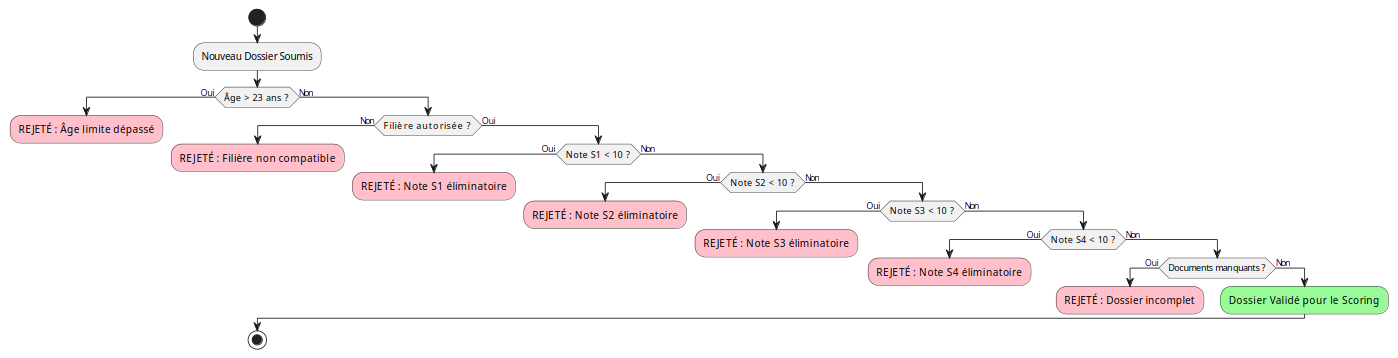
\includegraphics[width=\textwidth]{media/image11.png}
\caption{Fonctionnement du moteur de rejet automatique}
\label{fig:rejection-engine}
\end{figure}

\subsection{Journalisation des rejets}
Chaque rejet automatique génère un enregistrement HistoriqueAction contenant le motif précis de rejet, la règle déclenchée et l'horodatage. Le statut du dossier passe à REJETE\_AUTO et le candidat est notifié automatiquement par email.

\section{Algorithme de scoring pondéré par filière}
\subsection{Principe général}
Le scoring repose sur une pondération configurable par filière. Chaque filière définit des coefficients par catégorie de matières. Les moyennes semestrielles du candidat sont regroupées par catégorie via le fuzzy matching, puis pondérées selon les coefficients de la filière cible.

\subsection{Coefficients des quatre filières}
Le moteur de scoring applique les pondérations suivantes sur les catégories de matières extraites, en fonction de la filière choisie par le candidat :

\begin{table}[htbp]
\centering
\caption{Matrice des pondérations par filière}
\label{tab:ponderations}
{\small
\begin{tabular}{p{1.5cm} p{1.5cm} p{1.5cm} p{2cm} p{2cm} p{2cm} p{1.5cm}}
\toprule
\textbf{Filière} & \textbf{INFO} & \textbf{MATH} & \textbf{ELEC\_AUTO} & \textbf{CHIMIE\_BIO} & \textbf{RESEAUX\_BD} & \textbf{LANGUES} \\
\midrule
TDI & 35\% & 30\% & 25\% & --- & --- & 10\% \\
IACS & 40\% & 35\% & --- & --- & 15\% & 10\% \\
IAA & 10\% & 20\% & --- & 60\% & --- & 10\% \\
G2ER & 15\% & 30\% & 25\% & 30\% & --- & --- \\
\bottomrule
\end{tabular}
}
\end{table}

\subsection{Formule de calcul du score dossier}
Pour chaque filière $F$, le score dossier $S_d$ est calculé comme suit :

\begin{equation}
S_d(F) = \sum_{i=1}^{n} w_i(F) \times M_i
\label{eq:score_dossier}
\end{equation}

Où :
\begin{itemize}
\item $w_i(F)$ : poids de la catégorie de matière $i$ pour la filière $F$
\item $M_i$ : moyenne du candidat dans la catégorie $i$ (obtenue par fuzzy matching)
\item Si une catégorie indispensable n'est pas détectée, le moteur applique la moyenne générale comme fallback et marque le dossier comme SUSPECT
\end{itemize}

\begin{figure}[htbp]
\centering
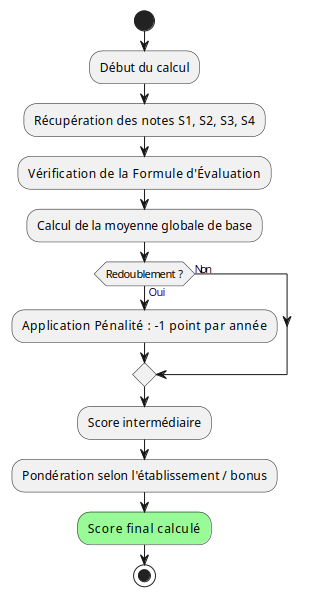
\includegraphics[width=0.4\textwidth]{media/image13.png}
\caption{Processus de calcul du score pondéré}
\label{fig:scoring-process}
\end{figure}

\subsection{Bonus de mention et coefficient diplôme}
Le score brut est enrichi par deux mécanismes de bonification :

\begin{table}[htbp]
\centering
\caption{Bonus de mention}
\label{tab:bonus-mention}
\begin{tabular}{p{5cm} p{4cm}}
\toprule
\textbf{Mention} & \textbf{Bonus} \\
\midrule
Très Bien ($\geq$ 16) & +2.0 points \\
Bien ($\geq$ 14) & +1.5 points \\
Assez Bien ($\geq$ 12) & +1.0 point \\
Passable ($\geq$ 10) & +0.0 point \\
\bottomrule
\end{tabular}
\end{table}

Un coefficient multiplicateur est appliqué selon le type de diplôme :

\begin{table}[htbp]
\centering
\caption{Coefficients par type de diplôme}
\label{tab:coefficient-diplome}
\begin{tabular}{p{7cm} p{4cm}}
\toprule
\textbf{Type de diplôme} & \textbf{Coefficient} \\
\midrule
DUT / BTS (spécialité correspondante) & $\times$1.00 \\
Licence (spécialité correspondante) & $\times$1.00 \\
Autre diplôme reconnu & $\times$0.80 \\
\bottomrule
\end{tabular}
\end{table}

\subsection{Formule du score final}
Le score final intègre la note de l'épreuve écrite selon la formule :

\begin{equation}
\text{Score\_final} = (\text{Score\_dossier} \times 0.40) + (\text{Note\_épreuve\_normalisée} \times 0.60)
\label{eq:score_final}
\end{equation}

En cas d'égalité de score final, le départage se fait par : (1) la note d'épreuve écrite, (2) la moyenne générale du dossier, (3) la date de soumission.

\section{Pipeline OCR et Fuzzy Matching}
\subsection{Extraction OCR}
Le pipeline de traitement automatique des relevés de notes s'appuie sur les bibliothèques pdfplumber (pour les PDF natifs) et pytesseract (pour les documents scannés). Le texte brut est extrait puis soumis à un processus de nettoyage.

\begin{figure}[htbp]
\centering
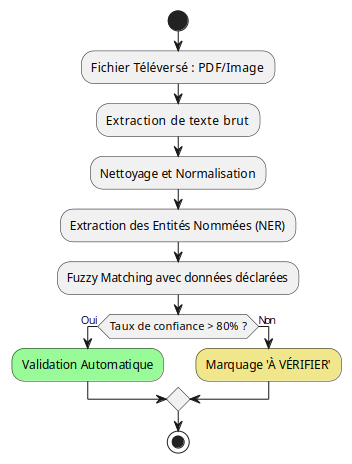
\includegraphics[width=0.4\textwidth]{media/image15.png}
\caption{Pipeline OCR et traitement des relevés de notes}
\label{fig:ocr-pipeline}
\end{figure}

\subsection{Nettoyage du bruit OCR}
Une fonction spécialisée filtre les erreurs fréquentes d'OCR sur les chiffres et les caractères :

\begin{table}[htbp]
\centering
\caption{Corrections automatiques du bruit OCR}
\label{tab:corrections-ocr}
\begin{tabular}{p{5cm} p{5cm}}
\toprule
\textbf{Caractère OCR} & \textbf{Correction} \\
\midrule
O (lettre) & 0 (chiffre) \\
l (lettre L min) & 1 (chiffre) \\
S (lettre) & 5 (chiffre) \\
I (lettre I maj) & 1 (chiffre) \\
\bottomrule
\end{tabular}
\end{table}

Les textes sont également normalisés : suppression des accents, passage en minuscules, suppression des caractères spéciaux.

\subsection{Fuzzy Matching des matières}
L'algorithme utilise la bibliothèque fuzzywuzzy pour comparer les noms de matières extraits par OCR avec un dictionnaire de catégories standardisées. Le processus :
\begin{itemize}
\item Chaque nom de matière extrait est comparé à toutes les entrées du dictionnaire
\item La fonction \texttt{fuzz.token\_sort\_ratio} calcule un score de similarité entre 0 et 100
\item Un seuil strict de 80\% est appliqué : seules les correspondances au-dessus sont retenues
\item Les catégories standardisées sont : MATH, INFO, CHIMIE\_BIO, ELEC\_AUTO, RESEAUX\_BD, LANGUES
\end{itemize}

Exemple : "Mathématiques pour l'ingénieur" $\rightarrow$ MATH (similarité 92\%)

Exemple : "Algorithmique et structures de données" $\rightarrow$ INFO (similarité 85\%)

\subsection{Scoring avec fallback}
Les notes extraites sont regroupées par catégorie standardisée. Si une catégorie indispensable à la filière n'est pas détectée par le fuzzy matching, le moteur applique la moyenne générale du candidat comme valeur de remplacement (fallback) et marque automatiquement le dossier comme SUSPECT pour vérification manuelle par le responsable.

\section{Calcul automatique des mentions}
La mention est calculée automatiquement dans la méthode \texttt{save()} du modèle NoteSemestre. La validation stricte impose que les moyennes soient dans la plage [10.00, 20.00]. Toute valeur hors plage déclenche une ValidationError Django.

Le champ mention est déclaré avec editable=False pour empêcher toute modification manuelle. Il est recalculé à chaque sauvegarde selon les seuils LMD définis précédemment dans la section 1.3.3.

\section{Conclusion}
Ce chapitre a présenté les algorithmes au cœur de la plateforme : le moteur de règles de rejet à 7 types, le scoring pondéré par filière avec ses formules mathématiques, et le pipeline OCR avec fuzzy matching. Ces mécanismes garantissent un traitement automatisé, fiable et transparent des candidatures. Le chapitre suivant détaillera l'implémentation, la gestion de l'asynchronisme et les tests.
